% DOCUMENTO PRINCIPAL

% Este es el fichero principal de este repositorio. No se recomienda editarlo.
% Modifica las plantillas incluidas en los directorios:
% - secciones
% - tablas
% - algoritmos

\documentclass[final,a4paper,11pt,twoside]{class_diss}

\usepackage[full]{textcomp}
\usepackage{graphicx}
\usepackage{amsmath}
\usepackage{amsxtra}
\usepackage{amssymb}
\usepackage{amsthm}
\usepackage{latexsym}
\usepackage{setspace}
\usepackage[margin=3cm]{geometry}
\usepackage[titles]{tocloft}
\usepackage{latexsym}
\usepackage{fancyhdr}
\usepackage{emptypage}
\usepackage[svgnames,dvipsnames,usenames,table,xcdraw]{xcolor}
\usepackage{tikz}
\usepackage[toc,acronym,nonumberlist,xindy={language=spanish-traditional},sanitize=none]{glossaries}
\usepackage[scaled]{helvet}
\usepackage[utf8]{inputenc}
\usepackage[T1]{fontenc}
\usepackage[spanish,es-tabla]{babel}
\usepackage[explicit]{titlesec}
\usepackage{newtxtext}
\usepackage{newtxmath}
\usepackage{stmaryrd}
\usepackage{bbold}
\usepackage[ruled,vlined]{algorithm2e}
\usepackage{algorithmic}
\usepackage{float}
\usepackage{url}
\usepackage{xspace}
\usepackage{booktabs}
\usepackage{multirow}
\usepackage{enumitem}
\usepackage{rotating}
\usepackage{pdflscape}
\usepackage{listings}
\usepackage{placeins}
\usepackage{flafter}

\theoremstyle{definition}
\newtheorem{definition}{Teorema}[section]
\theoremstyle{remark}
\newtheorem*{remark}{Remark}
\DeclareMathOperator*{\argmax}{arg\,max}
\DeclareMathOperator*{\argmin}{arg\,min}
\definecolor{VIU}{RGB}{240, 90, 15}
\definecolor{DESTACADO}{RGB}{130, 34, 145}
\definecolor{CITA}{RGB}{0, 123, 194}

\renewcommand{\algorithmcfname}{Algoritmo}
\renewcommand{\acronymname}{Lista de Acr\'onimos}
\addto\captionsspanish{
    \renewcommand*{\acronymname}{Lista de Acr\'onimos}
}
\newcommand{\inhib}{\relbar\mapsfromchar}
\newcommand{\destacado}[1]{\color{DESTACADO}\textbf{#1}\color{black}\xspace}

\usetikzlibrary{shapes}
\newcommand*\circled[1]{\tikz[baseline=(char.base)]{
    \node[shape=diamond,fill=black!90,inner sep=1pt,minimum size=1cm] (char) {\textcolor{white}{\small\textbf{#1}}};}
}

\pagestyle{fancy}
\fancyhf{}
\fancyhead[LO]{}
\fancyhead[RE]{}
\fancyfoot[C]{}
\renewcommand{\headrulewidth}{0pt}

\fancypagestyle{plain}{
  \fancyhf{}
  \fancyfoot[C]{\circled{\thepage}}
  \renewcommand{\headrulewidth}{0pt}
}

\colorlet{chapnumcolor}{VIU}

\newcommand*{\chapnumfont}{%
  \usefont{T1}{jkp}{b}{n}%
  \fontsize{70}{90}%
  \selectfont%
}

\newcommand*{\chaptitlefont}{%
  \usefont{T1}{qhv}{b}{n}%
  \fontsize{22}{26}%
  \selectfont%
}

\titleformat{name=\chapter}
{\normalfont\huge\bfseries}
{\rlap{\parbox{\textwidth}{\filleft\chapnumfont\color{chapnumcolor}\thechapter}}}
{0pt}
{\rlap{\parbox{0.7\textwidth}{\filright\chaptitlefont #1}}}

\makeglossaries
% GLOSARIO

% Si quieres incluir un glosario y una lista de abreviaturas en tu Trabajo Fin de Máster,
% sigue las instrucciones indicadas en la siguiente URL:
% https://www.overleaf.com/learn/latex/glossaries

%\newacronym{gan}{GAN}{Red Generativa Antagónica o \textit{Generative Adversarial Network}}


\bibliographystyle{apa}

\usepackage[authoryear,sort&compress]{natbib}
\usepackage{hypernat}
\setcitestyle{authoryear}

\usepackage[pdftex,plainpages=false,pdfpagelabels]{hyperref}

\hypersetup{
    linktocpage=true,
    colorlinks=true,
    bookmarks=true,
    citecolor=CITA,
    urlcolor=CITA,
    linkcolor=CITA,
    citebordercolor={1 0 0},
    urlbordercolor={1 0 0},
    linkbordercolor={.7 .8 .8},
    breaklinks=true,
    pdfpagelabels=true,
    }

\setcounter{secnumdepth}{3}
\onehalfspacing
\renewcommand\familydefault{\sfdefault}

\begin{document}

%%%% Incluye la portada oficial%%%%
%% Archivo portada.docx

\begin{titlepage}
    \centering
    \vspace*{1cm}

    \includegraphics[width=0.4\textwidth]{figuras/viu.png}\par\vspace{1cm}

    {\scshape\LARGE Universidad Internacional de Valencia\par}
    \vspace{1cm}
    {\scshape\Large Máster en Inteligencia Artificial\par}
    \vspace{1.5cm}

    {\huge\bfseries Optimización de prótesis robóticas de bajo costo\par}
    \vspace{2cm}

    {\Large Autor: Diego Rodríguez Atencia\par}
    \vfill

    {\large Fecha: \today\par}

    \vspace{0.8cm}
    \begin{flushleft}
        \large Tutor: Dr.-Ing. José Luis Zárate Moya\par

\end{flushleft}
\end{titlepage}

%\cleardoublepage

% Escribe aquí tu frase favorita
%\null\vspace{\stretch{2}}
%{
%\hfill \begin{minipage}{8cm}
%\textsl{
%\begin{flushright}
%    Escribe aquí \\ tu frase favorita.
%\end{flushright}
%}

% E indica aquí su autor
%\begin{flushright}
%E indica aquí su autor
%\end{flushright}

%\end{minipage}
%}
%\vspace{\stretch{1}}


\pagenumbering{gobble}
% AGRADECIMIENTOS

\cleardoublepage

\normalfont{\huge{\bfseries{Agradecimientos}}}
\vspace{15ex}

% Escribe tus agradecimientos a continuación.
% Se recomienda separar cada párrafo con un \medskip.

%Me gustaría agradecer...
%\medskip

%También quiero destacar...
%\medskip

%Por último...

\cleardoublepage

\newpage
\pagenumbering{roman}
\setcounter{page}{1}

\pagestyle{fancy}
\fancyhf{}
\fancyhead[LO]{\leftmark}
\fancyhead[RE]{\rightmark}
\fancyfoot[C]{\circled{\thepage}}
\renewcommand{\headrulewidth}{0.4pt}

\pdfbookmark[0]{\contentsname}{contents}

\renewcommand{\cftchapleader}{\cftdotfill{\cftdotsep}}
\renewcommand{\cftchapfont}{\mdseries}
\renewcommand{\cftchappagefont}{\mdseries}

\tableofcontents
\listoffigures
\listoftables

\renewcommand{\listalgorithmcfname}{Índice de algoritmos}
\listofalgorithms
\addcontentsline{toc}{chapter}{Índice de algoritmos}

\newpage
\pagenumbering{arabic}
\setcounter{page}{1}

\cleardoublepage

\chapter*{Resumen}
\label{resumen}
\addcontentsline{toc}{chapter}{Resumen}

% Escribe aquí 

% INTRODUCCIÓN

\cleardoublepage

\chapter{Introducción}
\label{introduccion}

Existen en el mundo más de 30 millones de personas con amputaciones según la OMS e ISPO (2017) \citep{whodata1}, y se estima que cada año se producen entre 1,5 y 2 millones de amputaciones. Estas cifras reflejan la magnitud del problema de las amputaciones y la necesidad de soluciones efectivas para mejorar la calidad de vida de estas personas.

En España, se estima que hay entre 70.000 y 90.000 pacientes amputados según el SERMEF (2021) , mientras que en México alrededor de un millón de personas necesitan prótesis y cinco millones requieren alguna ayuda ortésica, INEGI (2020). A nivel global, un estudio de la Organización Mundial de la Salud (OMS) indica que la proporción de amputados en algunos países occidentales oscila entre el 0,5 y el 1,25\% de la población. 

La solución actual de prótesis ortopédicas es costosa y no siempre accesible para todos. En España, una persona necesitada de una prótesis de mano se enfrenta ante la disyuntiva de pagar una cantidad desórbitada por una prótesis funcional que le permita recuperar autonomía, o bien gastarse una cantidad media para una prótesis estética o mecánica. Las prótesis estéticas son más asequibles, pero no ofrecen funcionalidad, mientras que las prótesis mecánicas son más costosas y requieren un mantenimiento constante. Por otro lado, las prótesis biónicas son una opción avanzada, pero su coste es elevado y no están al alcance de todos.

En este contexto, el objetivo de este trabajo es desarrollar un sistema de control para una mano biónica que permita a los usuarios recuperar la funcionalidad y autonomía en sus actividades diarias. El sistema se basa en el uso de señales electromiográficas (EMG) para controlar los movimientos de la mano biónica, y su optimización adicional mediante el uso de cámaras con una visión esteroscópica, lo que permite una interacción más natural y eficiente con el entorno.


\section{Marco teórico}
\label{marco-teorico}

Existen tres tipos diferentes de prótesis ortopédicas:
\begin{itemize}
    \item \textbf{Prótesis estéticas:} Estas prótesis están diseñadas para parecerse a una extremidad natural, pero no ofrecen funcionalidad. Son más asequibles, pero no permiten al usuario realizar movimientos precisos.
    \item \textbf{Prótesis mecánicas:} Estas prótesis utilizan mecanismos simples para permitir algunos movimientos básicos, como abrir y cerrar la mano. Son más funcionales que las estéticas, pero requieren un mantenimiento constante.
    \item \textbf{Prótesis biónicas:} Estas prótesis avanzadas utilizan tecnología electrónica y sensores para imitar los movimientos naturales de una mano. Son las más costosas, pero ofrecen la mayor funcionalidad y autonomía al usuario.
\end{itemize}

Dado que las prótesis estéticas no ofrecen funcionalidad, se descartan del marco teórico de este trabajo. Por otro lado, existen numerosas iniciativas actuales que facilitan el acceso a prótesis mecánicas, como la iniciativa  \citep{openbionics2018}, que proporciona prótesis mecánicas a un coste reducido. Estas prótesis utilizan el remanente en la extremidad del usuario para controlar los movimientos de la mano. Esta es una solución viable para muchas personas que cuentan con un remanente funcional, pero no es adecuada para aquellos que no tienen suficiente remanente o que necesitan una mayor funcionalidad.



Sin embargo, las prótesis biónicas permiten una mayor funcionalidad y autonomía al usuario, ya que permiten la programación y el diseño de diferentes algoritmos que permiten reconocer con algo de precisión la intención del usuario. Hay numerosos trabajos que salen relacionados con el desarrollo de prótesis que utilizan señales eléctricas EMG, cambio en la topología de la piel, o incluso señales cerebrales para controlar los movimientos de la mano biónica. 


Diseñar una prótesis biónica es un problema altamente complejo, en el que se busca maximizar la funcionalidad de la prótesis, atendiendo a las siguientes variables simultáneamente:
\begin{itemize}
    \item \textbf{Precisión y grados de libertad:} la prótesis debe ser capaz de tener los suficientes grados de libertad para realizar movimientos mínimamente funcionales.
    \item \textbf{Fuerza:} la prótesis debe ser capaz de regular la fuerza necesaria en diferentes actividades, para diferentes tipos de agarre y superficies, además de evitar aplicar demasiada fuerza en objetos frágiles. 
    \item \textbf{Peso:} Un peso excesivo en la prótesis puede dificultar su uso por largos periodos de tiempo, limitando su uso.
    \item \textbf{Costo:} Un costo elevado puede limitar el acceso a la prótesis.
    \item \textbf{Consumo de energía:} Un consumo de energía elevado limitaría el tiempo posible de uso de la prótesis, pero sin un consumo de energía adecuado, no pueden utilizarse sensores avanzados o micronocontroladores que permitan un control preciso de la prótesis.
    \item \textbf{Facilidad de uso:} La prótesis debe ser fácil de usar y no requerir un aprendizaje complejo por parte del usuario.
\end{itemize}

Las diferentes iniciativas actuales para este desarrollo suelen sacrificar algunas de estas variables para priorizar otras.

Un ejemplo de prótesis biónica de bajo costo es el de \textbf{Unlimited tomorrow}, que utiliza un sistema de control basado en sensores de cambio de la topología del remanente de la extremidad del usuario. El costo de esta prótesis ronda los 10.000 dólares, lo que la hace más accesible que otras prótesis biónicas avanzadas. Representa una solución viable para muchas personas que necesitan una prótesis biónica, pero no pueden permitirse el alto costo de las prótesis biónicas avanzadas. Cuentan con una diferenciación de hasta 16 tipos de agarre, lo que permite al usuario realizar una amplia variedad de movimientos y tareas cotidianas.

Un problema en general con las prótesis biónicas de bajo costo es que no cuentan con un sistema de control avanzado que permita al usuario realizar movimientos precisos y naturales. Por ejemplo, existen ciertos trabajos  \citep{emgcontrolled} que revisan diferentes enfoques para el control de prótesis biónicas utilizando señales EMG, pero no se centran en el desarrollo de sistemas de control avanzados que permitan al usuario realizar movimientos precisos y naturales.

La aplicación de técnicas de aprendizaje por refuerzo profundo para el control de prótesis bionicas es un campo de investigación activa, donde el mayor reto es la falta de datos de entrenamiento y la necesidad en muchos casos de un entorno simulado para entrenar los modelos. Aunque se han aplicado técnicas de aprendizaje supervisado, el hecho de que una prótesis necesita control en tiempo real de el movimiento y la fuerza aplicada, en entornos complejos y con estímulos ambiguos, hace que este sea complicado de aplicar. 

\medskip

\section{Estado del arte}
\label{estado-del-arte}


Se puede encontrar una revisión del estado del arte en el campo de las prótesis biónicas muy completa en el artículo \citep{bionicreview2023}, donde se contempla las variadas tecnologías utilizadas para el control de prótesis robóticas en el brazo. En este artóculo, pueden apreciarse los diferentes inputs usados por las prótesis:
\begin{itemize}
    \item \textbf{Señales electromiográficas (EMG):} Estas señales se obtienen a partir de la actividad eléctrica de los músculos y se utilizan para controlar los movimientos de la mano biónica. Son una de las formas más comunes de control en prótesis biónicas.
    \item \textbf{Sensores de fuerza (FMG):} Reciben señales del usuario empleando señales físicas producidas por el músculo. Un buen ejemplo de prótesis que utiliza este sistema de controle es \href{https://www.unlimitedtomorrow.com/about-unlimited-tomorrow/}{Unlimited tomorrow} que utiliza sensores de cambio de la topología del remanente de la extremidad del usuario para controlar los movimientos de la mano biónica.
    \item \textbf{Sensores de vibración (MMG):} Permiten reconocer la activación residual de los músculos mediante ligeras vibraciones.
    \item \textbf{Sensores de cambios de impedancia (EIT):} Estos sensores miden la impedancia eléctrica de los músculos y se utilizan para controlar los movimientos de la mano biónica.
    \item \textbf{Sensores de señales cerebrales (EEG):} Estos sensores miden la actividad eléctrica del cerebro y se utilizan para controlar los movimientos de la mano biónica. Son una forma avanzada de control, pero requieren un procesamiento complejo y no son tan comunes como las señales EMG. Un buen ejemplo de artículo que ha tenido cierto éxito con este tipod de sensores es \citep{labeegprosthesis2023}, donde se utilizó un dispositivo de toma de señales EEG superficiales para controlar una mano biónica.
\end{itemize}

Una imagen ilustrativa de los diferentes tipos de sensores utilizados en prótesis biónicas puede verse en la figura \ref{figuras/review2023.png}.
\begin{figure}[H]
    \centering
    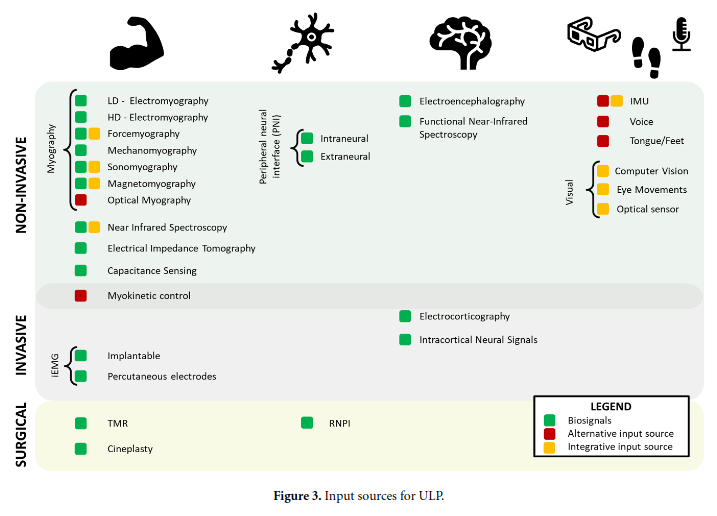
\includegraphics[width=0.8\textwidth]{figuras/review2023.png}
    \caption{Tipos de sensores utilizados en prótesis biónicas. Fuente: \citep{bionicreview2023}.}
    \label{figuras/review2023.png}
\end{figure}




\textit{Automatic Grasp Selection using a Camera in a Hand Prosthesis} \citep{automgrasp2016} demuestra que el uso de una cámara para la selección automática de agarres en una mano biónica es una solución viable y efectiva, pero no se centra en el desarrollo de un sistema de control avanzado que permita al usuario realizar movimientos precisos y naturales, sin centrarse en proporcionar una solución que involucre la complejidad a la hora de proporcionar una agarre preciso, sin establecer demasiada fuerza ni poca fuerza.

El trabajo de \citet{blais2025vision} propone la creación de una exoesqueleto con una cámara para rehabilitación, detallando problemas de implementación y complicaciones técnicas relacionadas con el consumo de energía adicional debido a la cámara. 

En \textit{Vision Controlled Sensorized Prosthetic Hand} \citep{sarker2024vision} , los investigadores logran implementar una prótesis biónica con un sistema de control basado en visión por cámara, que perimite decidir automáticamente el agarre a utilizar en función del objeto que se va a manipular. Este trabajo supone la demostración de que el input visual mejora destacablemente la precisión y adaptabilidad de los agarres de la mano biónica. Sin embargo, el usuario pierde el control sobre el agarre, quedando completamente a merced de la cámara y el algoritmo usado para la selección de control. Construyendo la prótesis, comentan adicionalmente complicaciones que surgen al integrar la cámara, como el consumo de energía adicional y la necesidad de añadir más poder de procesamiento para el algoritmo de detección de imágenes, lo que puede incrementar el peso y costo de la prótesis.

En \textit{Designing Prosthetic Hands With Embodied Intelligence: The KIT Prosthetic Hands} \citep{kit2021prosthetic} , los investigadores incorporan de forma exitosa una cámara en una mano biónica, involucrando además señales EMG y realizando incluso pruebas sobre pacientes reales, y recogiendo resultados acerca del éxito que han tenido con algunas tareas. Este trabajo demuestra el éxito a la hora de integrar la señal EMG del remanente y el input visual de la cámara.

Un trabajo similar al anterior es \textit{Design of an Affordable Prosthetic Arm Equipped with DeepLearning Vision-Based Manipulation} \citep{prosthesisdeeplearning}, trabajo en el que se propone una prótesis similar, que utiliza señales EMG y visión por cámara para el control de una mano biónica. En este artículo, utilizan técnicas de aprendizaje por refuerzo profundo en Mujoco para simular la mano biónica y validar los resultados obtenidois.

El aprendizaje por refuerzo profundo ha sido aplicado con éxito a el desarrollo de la destreza en manipulación de objetos en entornos simulados, como en el artículo \textit{Deep reinforcement learningfor dexterous hand manipulation} \citep{deepdexterous}, donde se demuestra que el aprendizaje por refuerzo profundo puede ser utilizado para entrenar un agente a manipular objetos con una mano biónica en un entorno simulado. Cabe destacar la involucración del aprendizaje por refuerzo inverso, dada la dificultad a la hora de definir una función de recompensa adecuada para el control de la mano biónica. Esta simulación fué evaluada en Mujoco, un simulador de física que involucra la simulación de cuerpos rígidos y suaves, y que permite simular el movimiento de la mano biónica en un entorno controlado.


\medskip

% Define los acrónimos en el fichero secciones/glosario.tex
% Define la bibliografía en el fichero bibliografia.bib

% OBJETIVOS

\cleardoublepage

\chapter{Objetivos}
\label{objetivos}



\medskip
\begin{enumerate}[label=\destacado{\arabic*.}]
  \setlength\itemsep{1em}
  \item \textbf{Objetivo parcial 1.} Generar un dataset personalizado de pares de activaciones EMG + Imágenes estereoscopicas parametrizables para el entrenamiento de prótesis de mano robótica.
    Se utilizará el entorno de simulación Mujoco, y el dataset GRAB para simular el gesto de agarre de objetos de un usuario. Las activaciones EMG del antebrazo se simularán utilizando el framework NeuroMotion \citep{ma2023neuromotion}, y las imágenes estereoscópicas se generarán a partir de la simulación del entorno con una cámara virtual.

  \item \textbf{Objetivo parcial 2.} Entrenar un modelo de aprendizaje por refuerzo profundo para la
    predicción de movimientos de mano robótica a partir de señales EMG y imágenes estereoscópicas, utilizando DDPG o PPO como algoritmos de entrenamiento.

  \item \textbf{Objetivo parcial 3.} Evaluar el rendimiento del modelo entrenado en un entorno simulado, comparando su eficacia con otros enfoques existentes en la literatura.
\end{enumerate}

% METODOLOGÍA

\cleardoublepage

\chapter{Metodología}
\label{metodologia}

% RESULTADOS Y DISCUSION 

\cleardoublepage

\chapter{Resultados y Discusión}
\label{resultados-y-discusion}

% CONCLUSIONES

%\chapter{Conclusiones}
%\label{conclusiones}

%\begin{enumerate}[label=\destacado{\arabic*.}]
%  \setlength\itemsep{1em}
%  \item Conclusión 1.

%  \item Conclusión 2.

%  \item Conclusión 3.
%\end{enumerate}

% LIMITACIONES Y PERSPECTIVAS DE FUTURO

\cleardoublepage

\chapter{Limitaciones y\\ Perspectivas de Futuro}
\label{limitaciones-y-futuro}


\cleardoublepage
\phantomsection

\printglossary[type=\acronymtype]
\printglossary

\appendix
% APÉNDIZES

% Escribe cada apéndize como si fuera un capítulo más.

%\chapter{Apéndize A}
%\label{apendize-a}

%\chapter{Apéndize B}
%\label{apendize-b}


\begin{singlespace}
\begin{footnotesize}
\begin{twocolumn}
\bibdata{bibliografia}
\bibliography{bibliografia}
\addcontentsline{toc}{chapter}{Bibliografía}
\end{twocolumn}
\end{footnotesize}
\end{singlespace}

\end{document}
